\documentclass{beamer}
 
\usepackage[frenchb]{babel}
\usepackage[T1]{fontenc}
\usepackage[utf8]{inputenc}

 
\usetheme{Warsaw}
  
\title{Stage au LIRMM : RollingCat}
\author{Noé LE PHILIPPE}
\institute{}
\date{\today}
\logo{
\includegraphics[height=5mm]{images/logo.png}}

\AtBeginSection[]
{
  \begin{frame}
  \frametitle{Sommaire}
  \tableofcontents[currentsection, hideothersubsections]
  \end{frame} 
}

\begin{document}

\begin{frame}
\titlepage
\end{frame}
	
\section{Présentation du sujet}
\begin{frame}
\frametitle{Présentation du sujet}

\begin{block}{Mission ?}
Réalisation d'un serious game
\end{block}

\pause

\begin{block}{Pour qui ?}
Les patients ayant subi un AVC
\end{block}

\pause

\begin{block}{Pourquoi ?}
Rééducation des membres supérieurs
\end{block}

\end{frame}

\subsection{Qu'est ce qu'un serious game}
\begin{frame}
\frametitle{Qu'est ce qu'un serious game}

\begin{block}{Définition}
Un serious game, ou jeu sérieux, est un jeu dont la finalité première n'est pas le divertissement, mais plutôt la formation, la rééducation, l'entraînement etc
\end{block}

\end{frame}

\subsection{Contraintes liées au public}
\begin{frame}
\frametitle{Contraintes liées au public}

\begin{block}{}
Accessible
\end{block}
\pause

\begin{block}{}
Adapté
\end{block}
\pause
\begin{block}{}
Amusant
\end{block}

\end{frame}
 
\subsection{Mise en place de la rééducation}
\begin{frame}
\frametitle{Mise en place de la rééducation}

\begin{block}{Matériel}

\begin{itemize}
\item Ordinateur connecté à internet
\item Tablette graphique de 100*50 cm
\item Souris accrochée à la main
\end{itemize}

\end{block}

\pause
\begin{block}{Rééducation}
Forcer le patient à effectuer certains mouvements des bras
\end{block}

\pause
\begin{block}{Encadrement}
Le patient est toujours sous la supervision d'un thérapeute
\end{block}

\end{frame}

\begin{frame}

\begin{columns}
	\begin{column}{0.5\textwidth}
		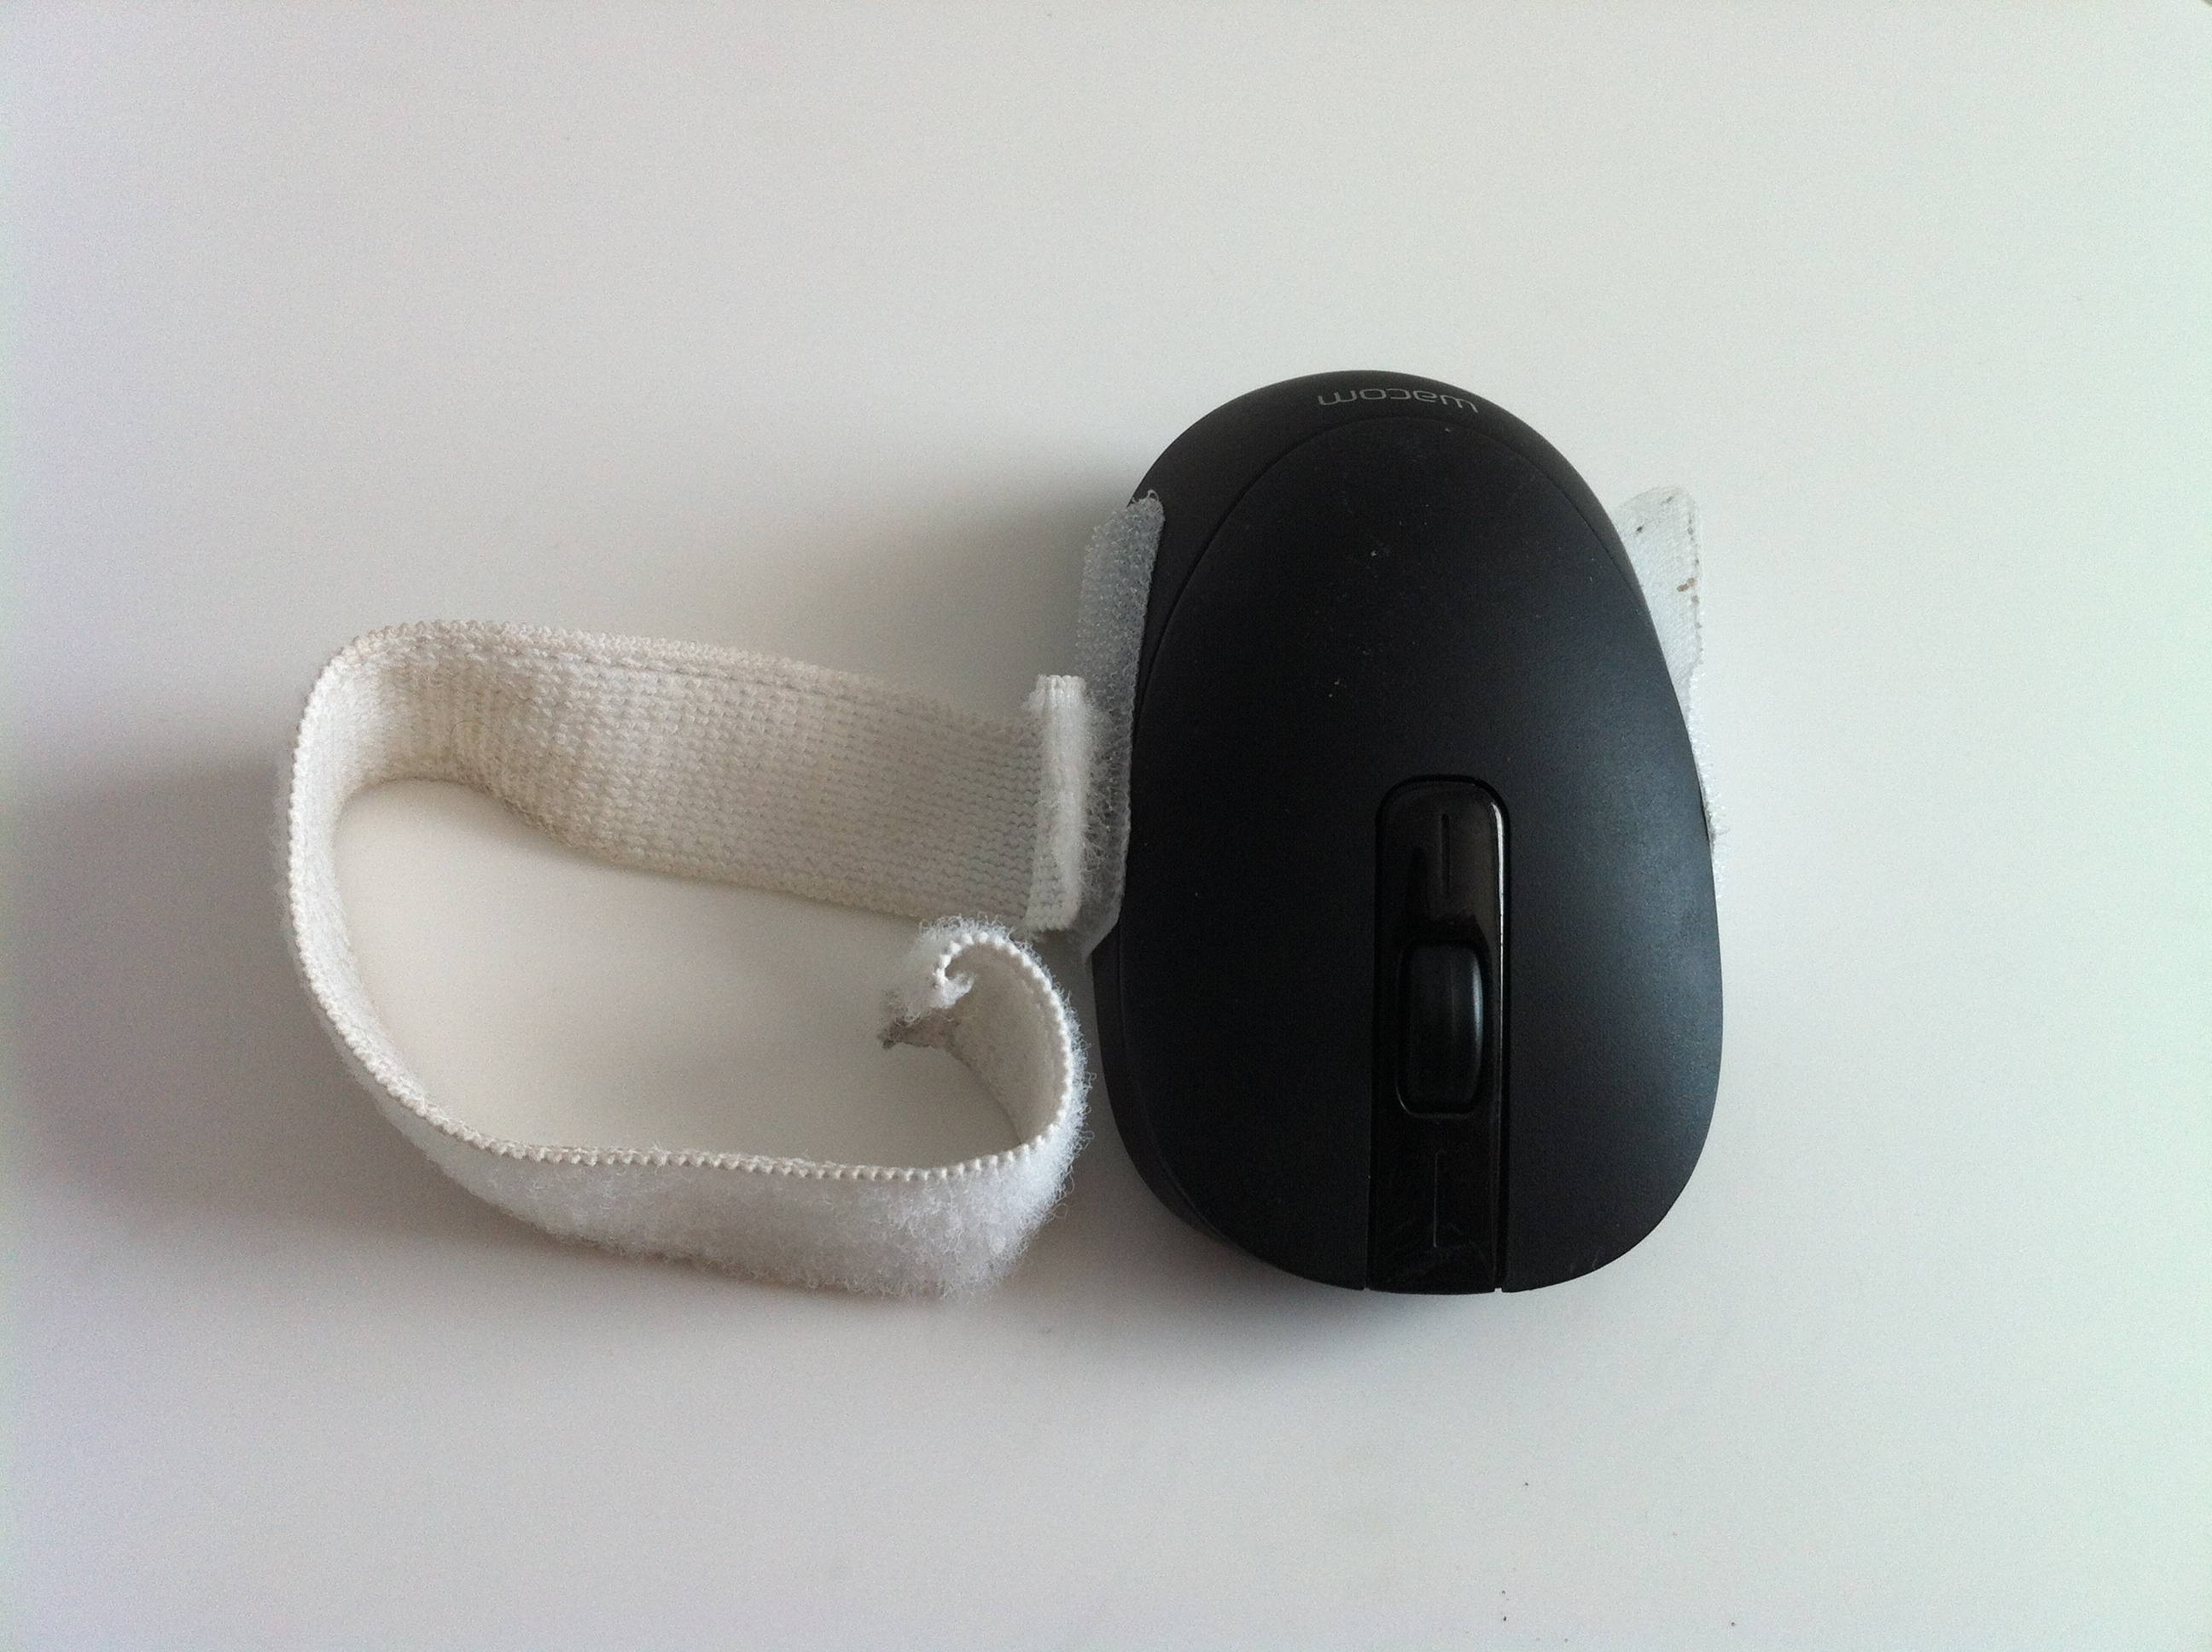
\includegraphics[scale=0.05]{images/souris.JPG}
	\end{column}
	\begin{column}{0.5\textwidth}
		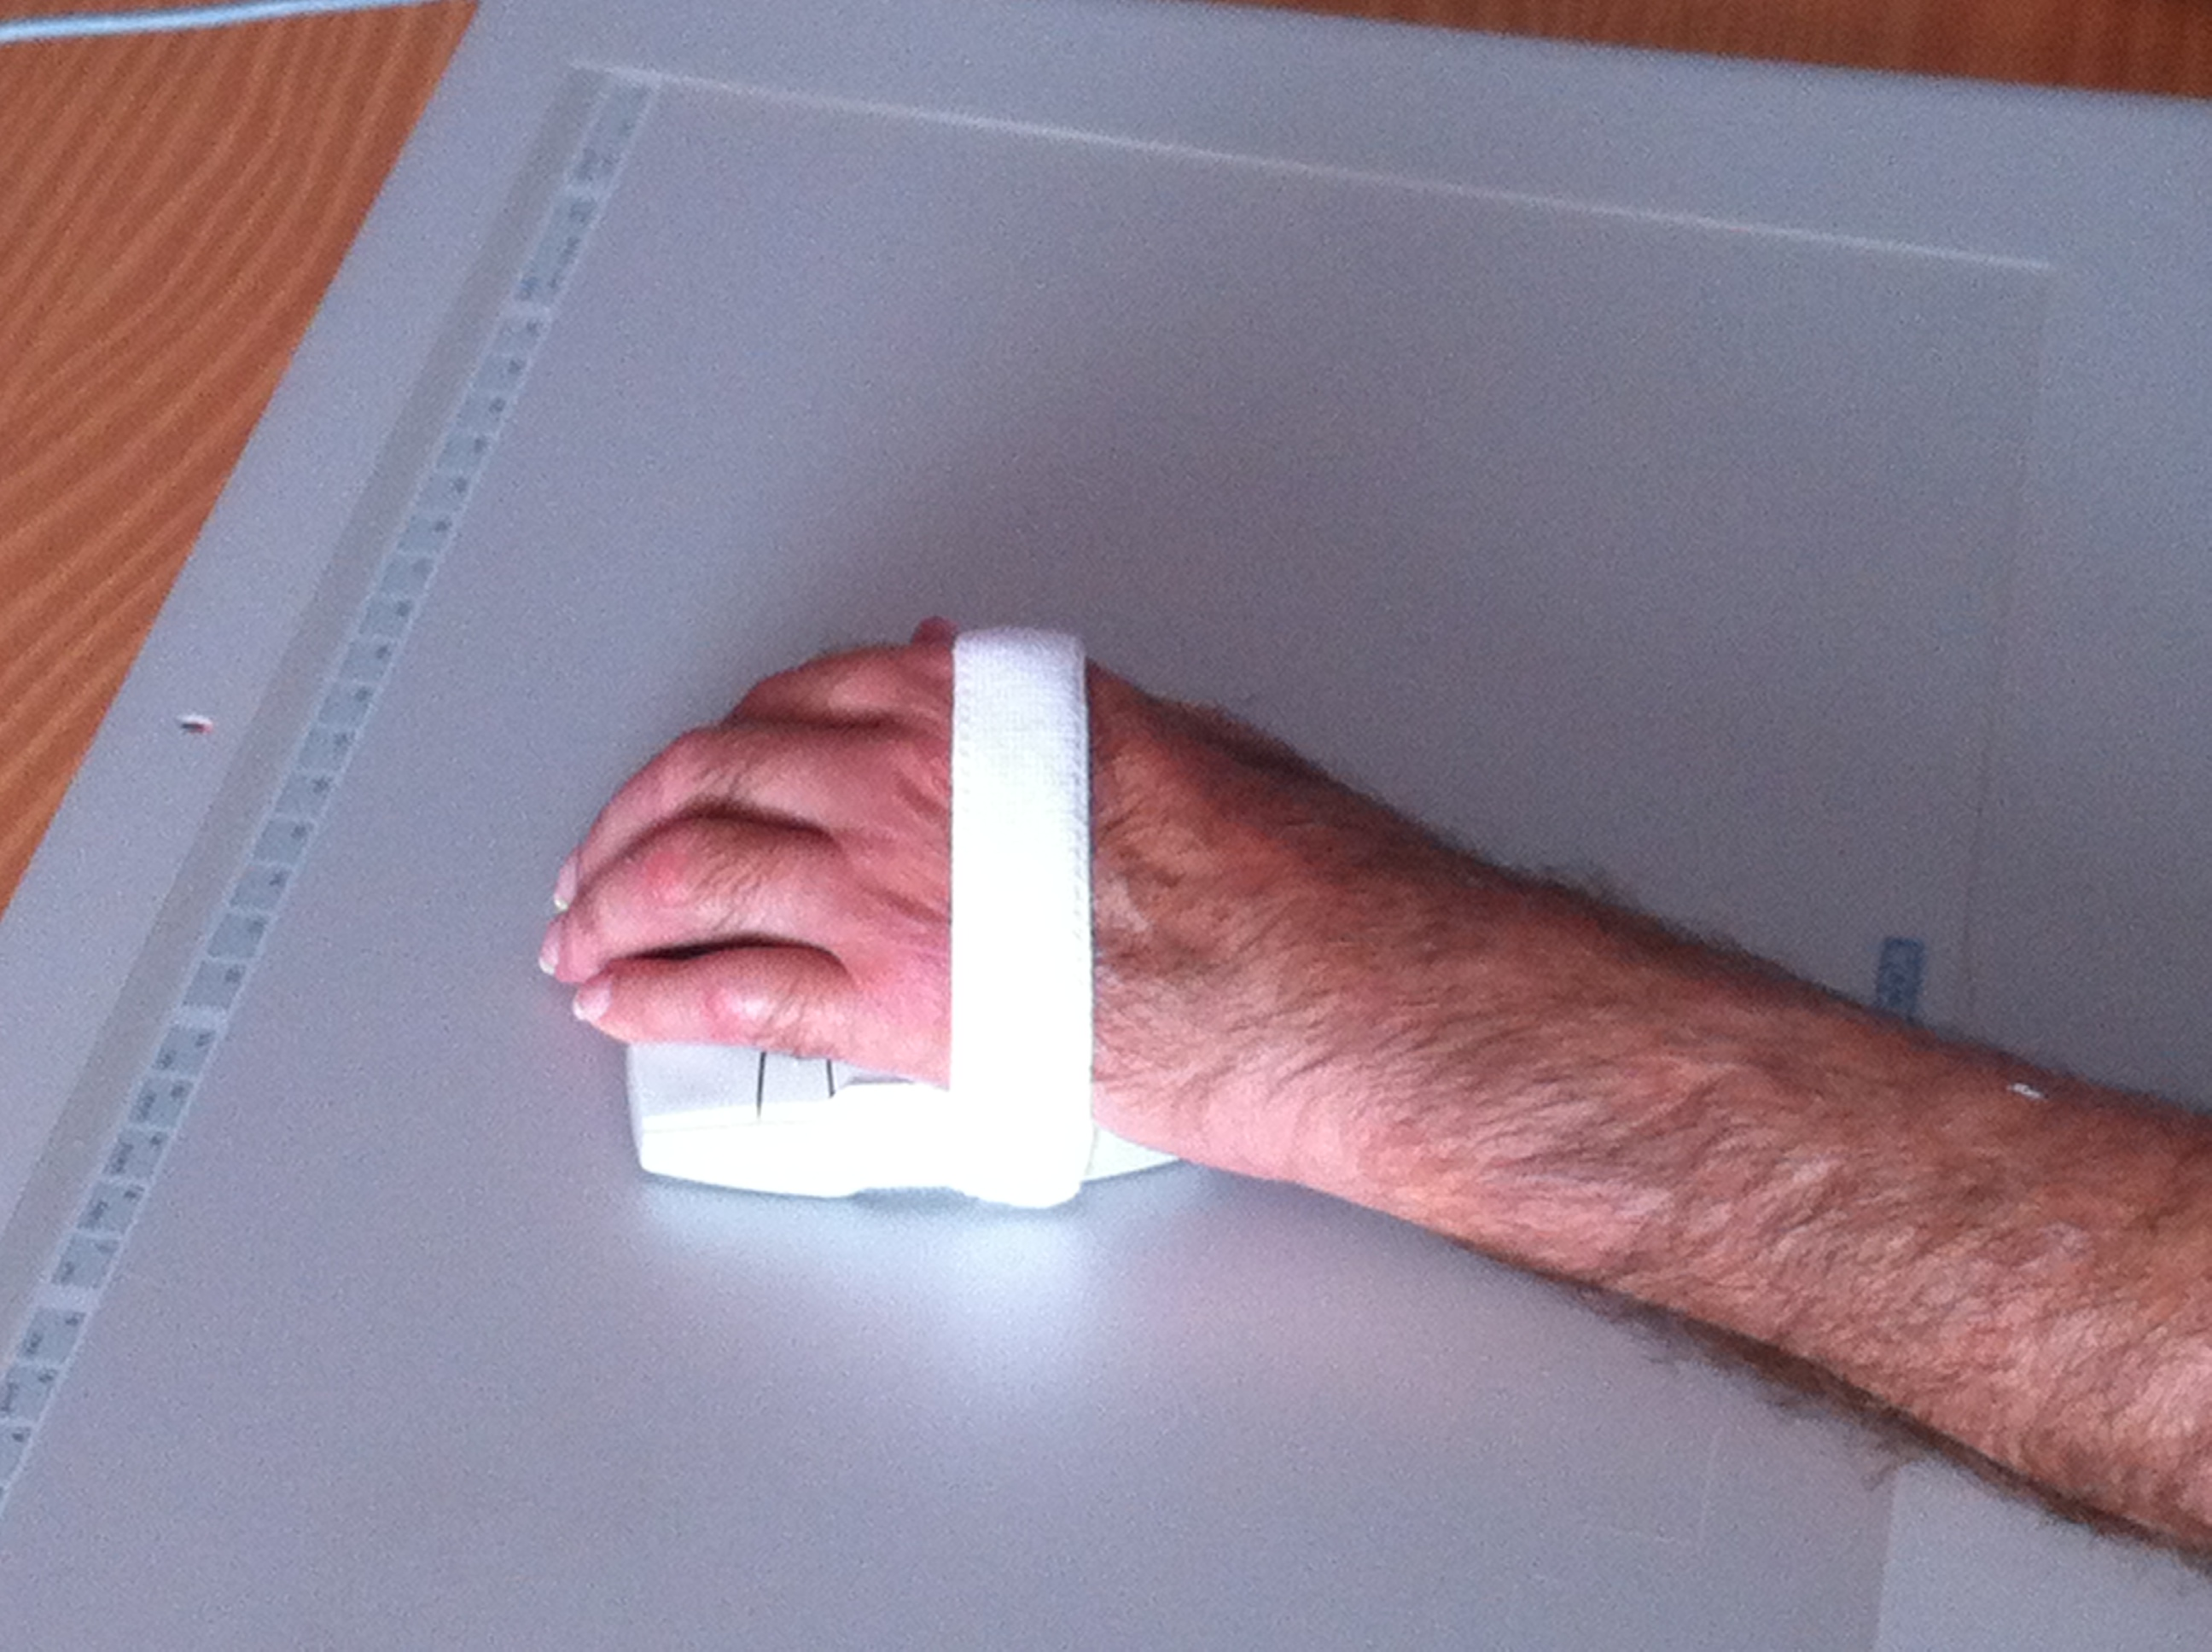
\includegraphics[scale=0.05]{images/main.JPG}
	\end{column}
\end{columns}

\end{frame}

\subsection{Vocabulaire}

\begin{frame}
\frametitle{Vocabulaire}

\begin{block}{Tâche de pointage}
Cible que le patient doit atteindre
\end{block}

\begin{block}{Zone d'habilité}
Espace que le patient est en mesure d'atteindre avec ses mains sur la tablette
\end{block}

\end{frame}

\section{Game Design Document}

\subsection{Principe de base du jeu}

\begin{frame}
\frametitle{Principe de base du jeu}
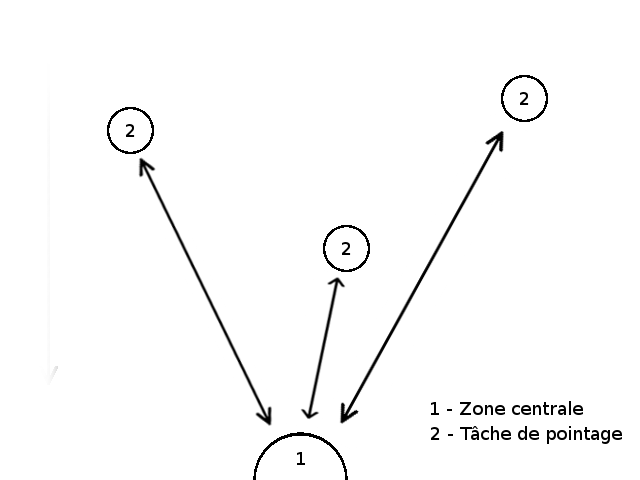
\includegraphics[scale=0.4]{images/gameplay.png}
\end{frame}

\begin{frame}
\frametitle{Principe de base du jeu}

\begin{block}{Structure du niveau}
	Découpé en plusieurs sous-parties : les \textbf{segments}
\end{block}
\pause
\begin{block}{Pourquoi être découpé ?}
Donner un objectif à court terme simple à atteindre 
\end{block}

\end{frame}


\subsection{Des concepts à la réalité}
\begin{frame}
\frametitle{Des concepts à la réalité}

\begin{block}{Les tâches de pointage}
\begin{itemize}
\item Les rendre obligatoires
\item Les rendre visuelles
\end{itemize}
\end{block}

\begin{block}{La zone centrale}
\begin{itemize}
\item L'intégrer au jeu
\item La rendre visuelle
\end{itemize}
\end{block}

\end{frame}

\begin{frame}
\frametitle{Des concepts à la réalité}

\begin{center}
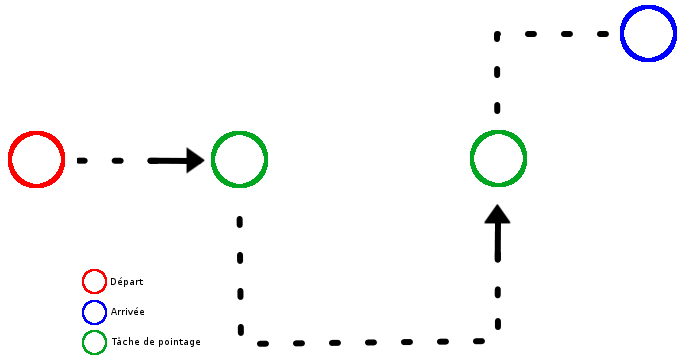
\includegraphics[scale=0.4]{images/path.png}
\end{center}
\end{frame}

\begin{frame}
\frametitle{Des concepts à la réalité}

\begin{center}
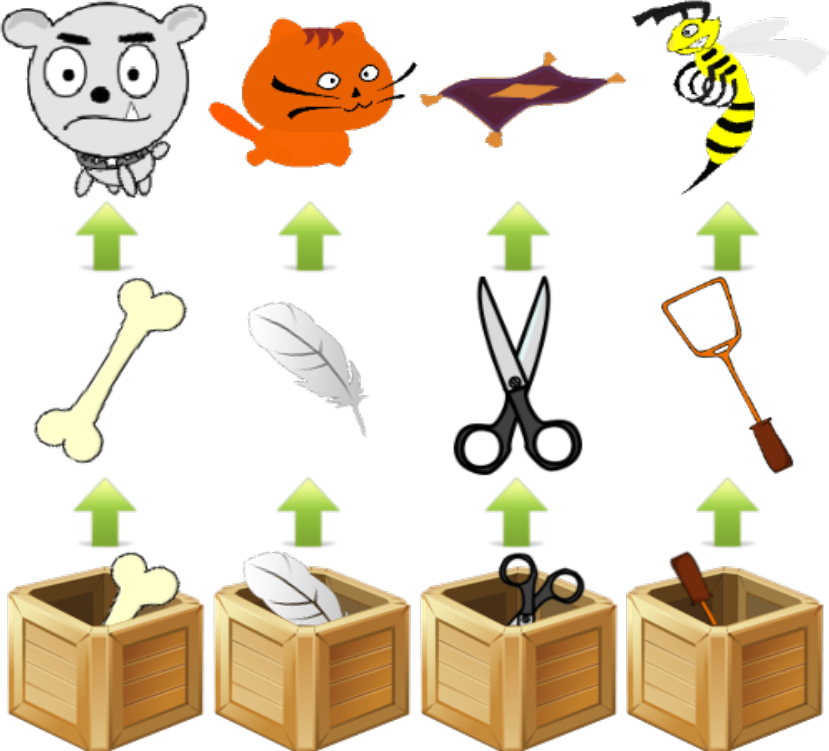
\includegraphics[scale=0.24]{images/esthetique.png}
\end{center}
\end{frame}

\subsection{Les éléments du décor}
\begin{frame}
\frametitle{Les éléments du décor}
Le chat va devoir se déplacer dans trois directions : le haut, le bas et la droite
\end{frame}

\begin{frame}
\frametitle{Les éléments du décor}


\begin{columns}
	\begin{column}{0.8\textwidth}
		\begin{block}{Vers le haut}
			Un ventilateur
		\end{block}
	\end{column}
	\pause
	\begin{column}{0.2\textwidth}
		
\includegraphics[scale=0.4]{images/fan.png}
	\end{column}
\end{columns}
\pause
\begin{columns}
	\begin{column}{0.8\textwidth}
		\begin{block}{Vers le bas}
			La gravité
		\end{block}
	\end{column}
	\begin{column}{0.2\textwidth}
	\end{column}
\end{columns}
\pause
\begin{columns}
	\begin{column}{0.8\textwidth}
		\begin{block}{Vers la droite}
			Le sol
		\end{block}
	\end{column}
	\pause
	\begin{column}{0.2\textwidth}
		
\includegraphics[scale=0.4]{images/groundblock.png}
	\end{column}
\end{columns}

\end{frame}

\subsection{Les rewards}
\begin{frame}
\frametitle{Les rewards}

\begin{columns}
	\begin{column}{0.8\textwidth}
		\begin{block}{Récompenser les efforts}
			Mettre en place une mesure visuelle pour le patient de ses efforts
		\end{block}
	\end{column}
	\pause
	\begin{column}{0.2\textwidth}
		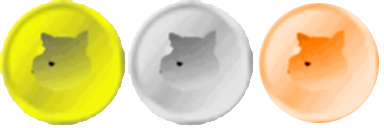
\includegraphics[scale=0.2]{images/coins.png}
	\end{column}
\end{columns}
\begin{columns}
	\pause
	\begin{column}{0.8\textwidth}
		\begin{block}{Apporter de la rejouabilité}
			Le patient pourra améliorer son score et se rendre compte de ses progrès
		\end{block}
	\end{column}
	\begin{column}{0.2\textwidth}
	\end{column}
\end{columns}

\end{frame}


\subsection{Le chemin de secours}

\begin{frame}
\frametitle{Le chemin de secours}

\begin{block}{Qu'est ce que le chemin de secours}
Un chemin alternatif que le chat empruntera en cas d'échec
\end{block}
\pause
\begin{block}{Pourquoi un chemin de secours}
\begin{itemize}
\pause
\item Ne pas s'arrêter en cas d'échec \pause
\item Éviter la frustration \pause
\item Continuer à évaluer les autres tâches
\end{itemize}
\end{block}

\end{frame}

\begin{frame}
\frametitle{Le chemin de secours}

\centering 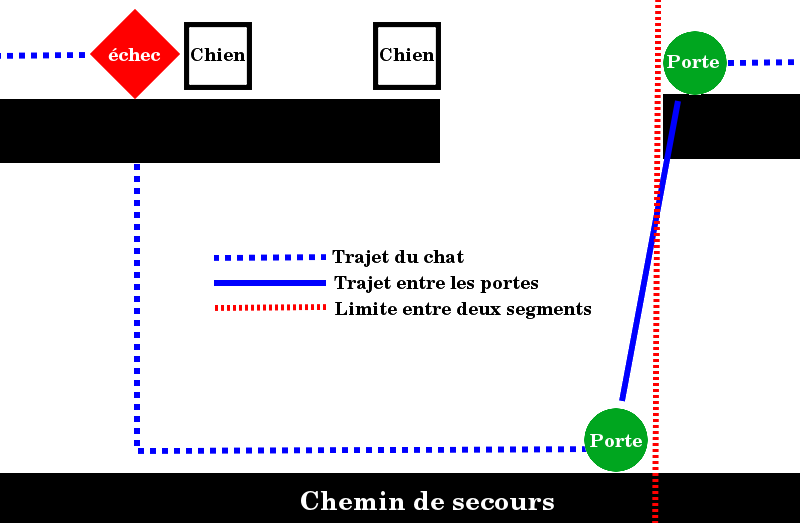
\includegraphics[scale=0.3]{images/secours.png}

\end{frame}


\subsection{Exemple de niveau basique}

\begin{frame}
\frametitle{Exemple de niveau basique}
\centering 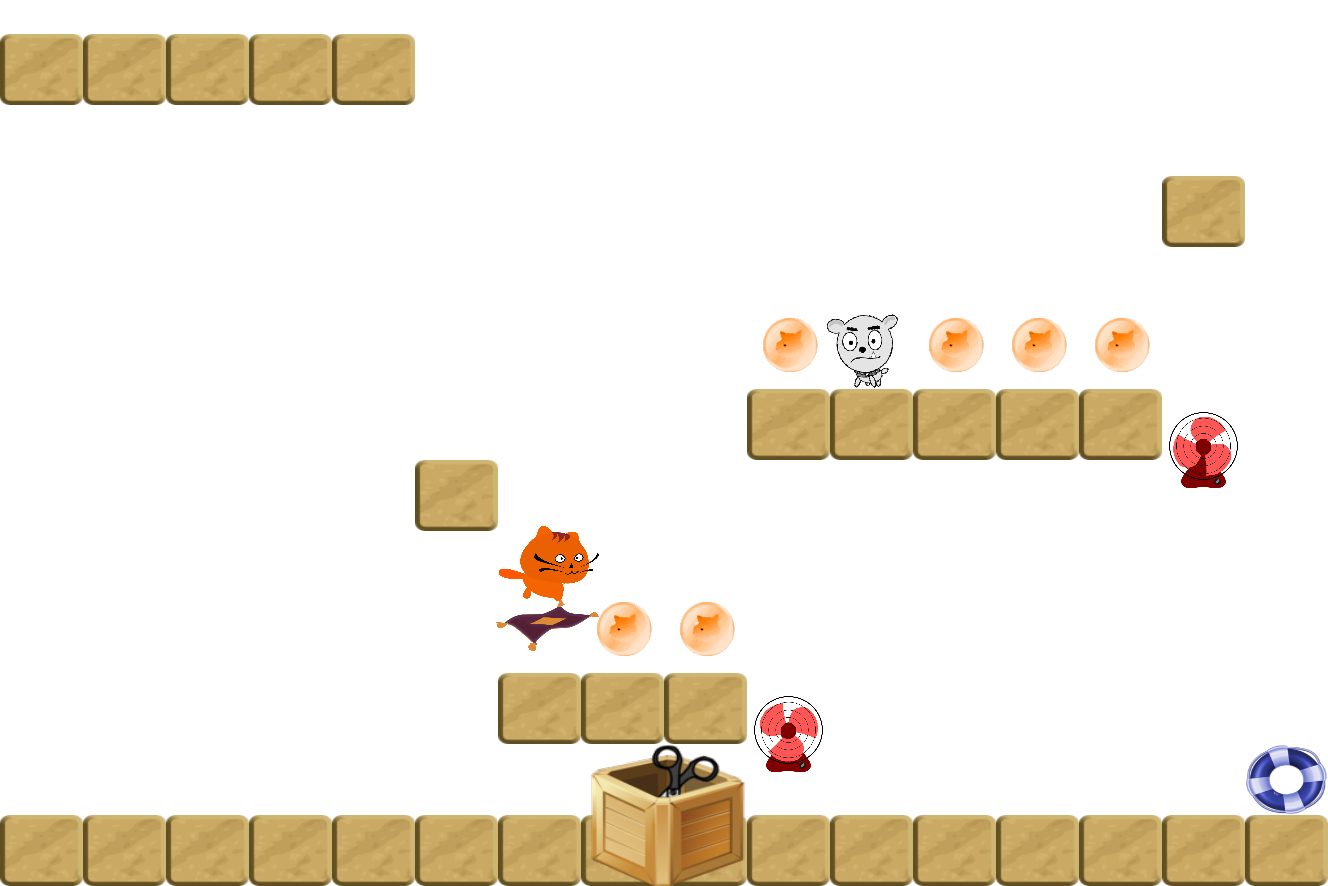
\includegraphics[scale=0.19]{images/simple_level.png}

\end{frame}

\section{Conception}
\subsection{UML du monde}

\begin{frame}
\frametitle{UML du monde}

\centering 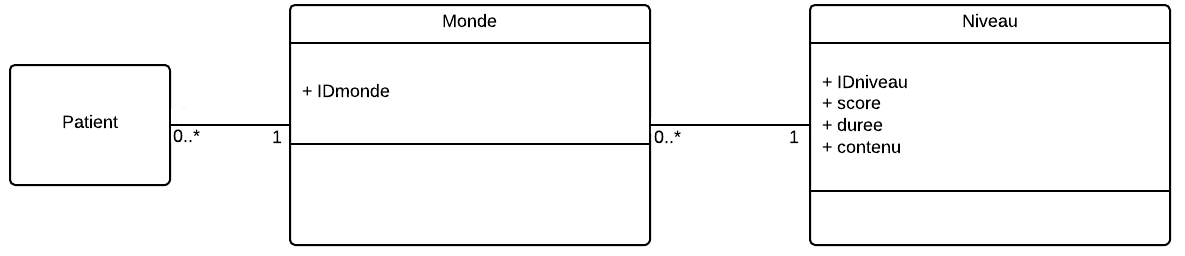
\includegraphics[scale=0.25]{images/uml_monde.png}

\end{frame}

\subsection{Architecture client-serveur}
\begin{frame}
\frametitle{Échanges entre le client et le serveur}
\centering 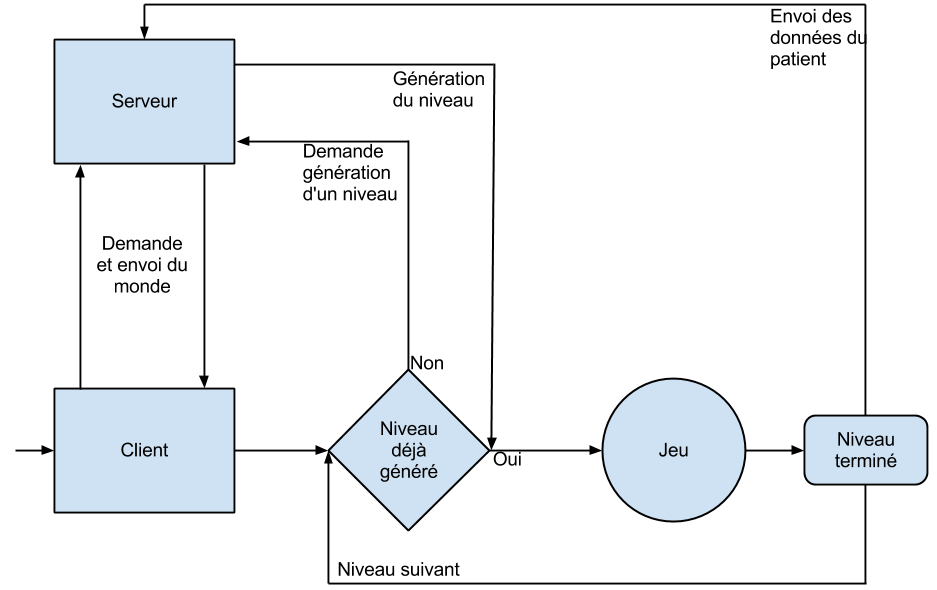
\includegraphics[scale=0.27]{images/client-serveur.png}

\end{frame}

\subsection{Adaptation}
\begin{frame}
\frametitle{Adaptation}

\begin{block}{Une double adaptation}
Le jeu dispose d'une double adaptation, une première coté serveur et une autre coté client
\end{block}

\end{frame}

\begin{frame}
\frametitle{Adaptation coté serveur}

\begin{block}{Comment ?}
Les capacités du patient sont évaluées grâce à l'évaluation en jeu
\end{block}

\end{frame}

\begin{frame}
\frametitle{Adaptation coté serveur : évaluation}

\centering 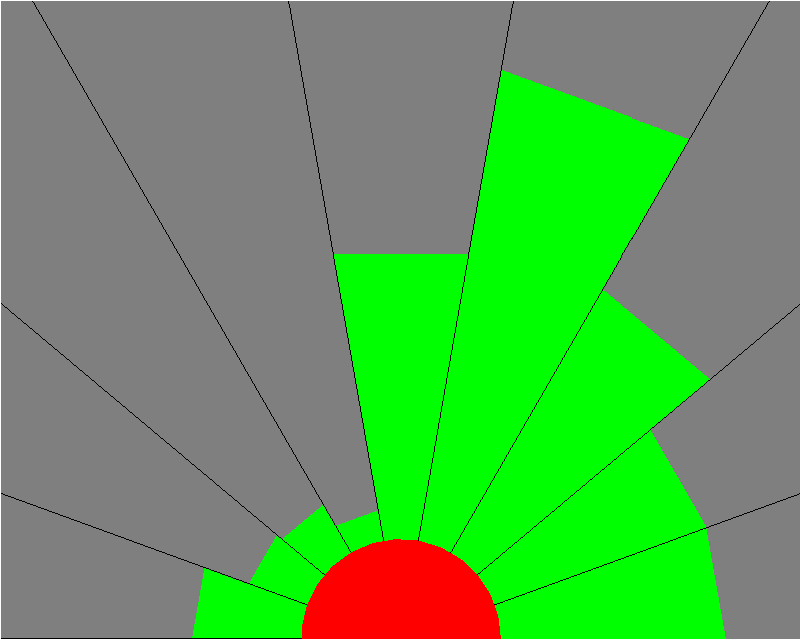
\includegraphics[scale=0.3]{images/assessment.png}

\end{frame}

\begin{frame}
\frametitle{Adaptation coté serveur : résultat en jeu}

\centering 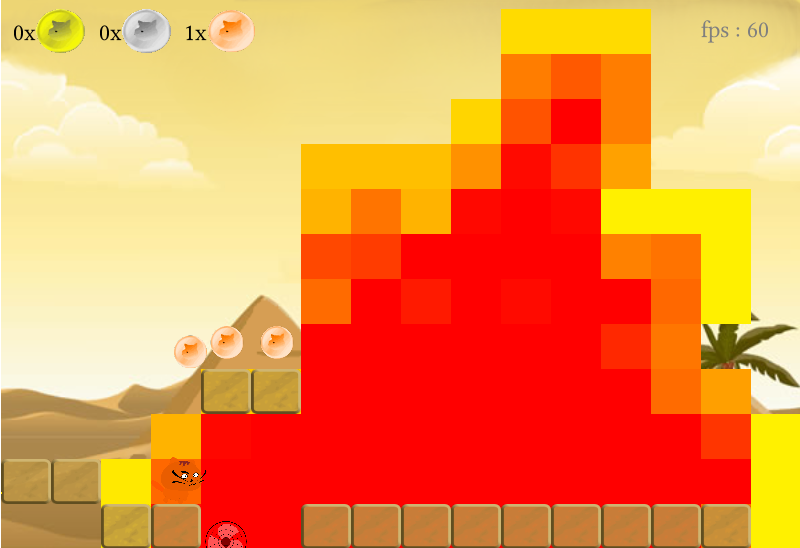
\includegraphics[scale=0.3]{images/abilityzone.png}

\end{frame}

\begin{frame}
\frametitle{Adaptation coté serveur : placement des tâches de pointage}

\begin{block}{Rouge}
Zone acquise, tâches de pointage uniquement dans un niveau facile
\end{block}

\begin{block}{Jaune - orange}
En cours d'acquisition, les tâches de pointage y seront placées en cas de niveau normal
\end{block}

\begin{block}{Sans couleur}
Non-acquis, les tâches de pointage y seront placées en cas de niveau difficile
\end{block}

\end{frame}

\begin{frame}
\frametitle{Adaptation coté client}
\begin{block}{Comment ?}
Le niveau est en fait composé de cinq sous-niveaux superposés, d'autant plus durs qu'ils sont hauts
\end{block}

\end{frame}

\begin{frame}
\frametitle{Adaptation coté client : cinq étages superposés}

\centering 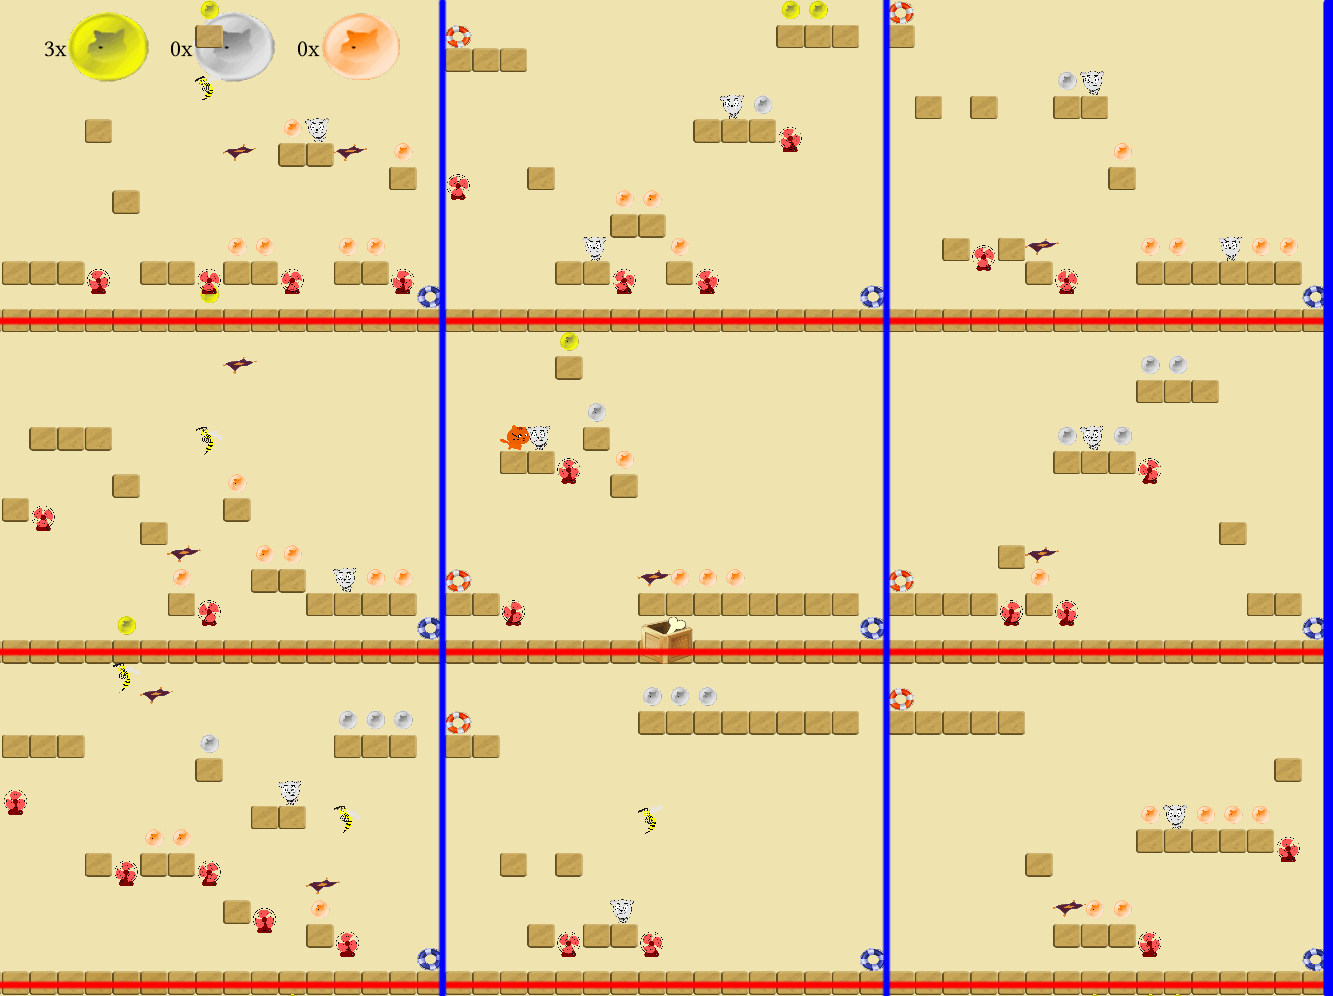
\includegraphics[scale=0.18]{images/3etages.png}

\end{frame}

\begin{frame}
\frametitle{Adaptation coté client : les portes}

\begin{block}{Déplacement horizontal}
Faire passer le chat au segment suivant
\end{block}
\pause	
\begin{block}{Déplacement vertical}
Faire passer le chat au bon étage selon les résultats du patient
\end{block}
\pause
\begin{block}{Adaptation}
L'adaptation se fait en choisissant le bon étage par rapport aux capacités du patient
\end{block}

\end{frame}

\subsection{Déplacements du chat}
\begin{frame}
\frametitle{Déplacements du chat : les états}
Les déplacements sont automatiques, ils sont calculés en fonction de l'état du chat
\pause
\begin{block}{Les états}
\begin{itemize}
\item FALLING
\item FLYING
\item HITTING
\item WALKING
\end{itemize}
\end{block}

\end{frame}

\begin{frame}
\frametitle{Déplacements du chat : calcul des états}
Les états dépendent de ce avec quoi le chat est en contact
\begin{block}{Quel élément}
\begin{itemize}
\item Rien : FALLING
\item Un ventilateur : FLYING
\item Une tâche de pointage : HITTING
\item Le sol : WALKING
\end{itemize}
\end{block}
\end{frame}

\begin{frame}
\frametitle{Déplacements du chat : mouvements en fonction des états}
Ce sont les états qui donnent ses déplacements au chat
\begin{block}{Les états}
\begin{itemize}
\item FALLING : un bloc vers le bas
\item FLYING : un bloc vers le haut
\item HITTING : on arrête tout mouvement
\item WALKING : un bloc vers la droite
\end{itemize}
\end{block}
\end{frame}

\subsection{La boîte}
\begin{frame}
\frametitle{La boîte : construction}
La boîte est remplie lors de la construction du niveau, les objets lui sont ajoutés en fonction de l'entité rencontrée. \\
Elle est composée de plusieurs sous-boîtes : une par segment


\end{frame}

\begin{frame}
\frametitle{La boîte : faire correspondre les objets avec le segment}


\begin{center}
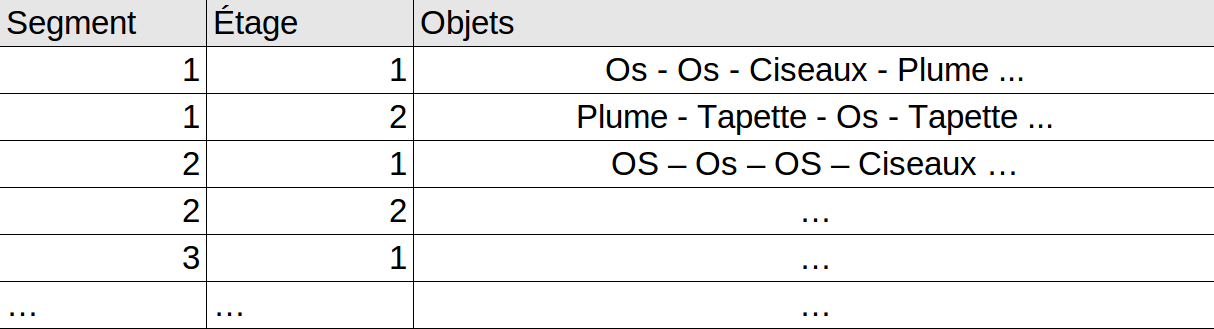
\includegraphics[scale=0.2]{images/boite.png}
\end{center}

Les entités ont toutes un couple étage/segment en fonction de leur position
Cela forme la clé qui permettra de retrouver la bonne boîte
\end{frame}

\begin{frame}
\frametitle{La boîte : faire correspondre les objets avec le segment}
Par exemple si le chat se trouve segment 2 étage 1, la clé sera 2-1
\begin{center}
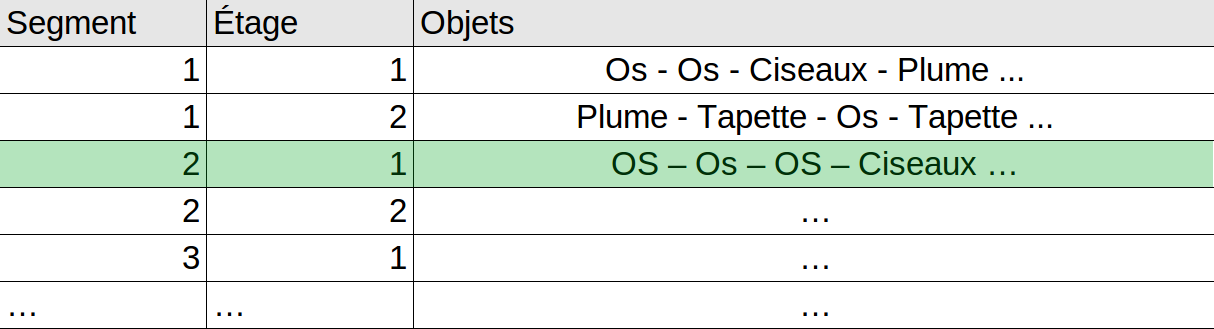
\includegraphics[scale=0.2]{images/boite_selected.png}
\end{center}
\end{frame}

\subsection{Plusieurs esthétiques : plusieurs jeux}
\begin{frame}
\frametitle{Plusieurs esthétiques}

\begin{block}{Une fabrique de jeux}
Une mécanique pour un nombre illimité de jeux
\end{block}

\begin{block}{Un jeu par esthétique}
Chaque esthétique est un jeu à part entière, avec un monde et des niveaux séparés des autres esthétiques
\end{block}
\end{frame}

\begin{frame}
\frametitle{Plusieurs esthétiques : le chat}
\begin{center}
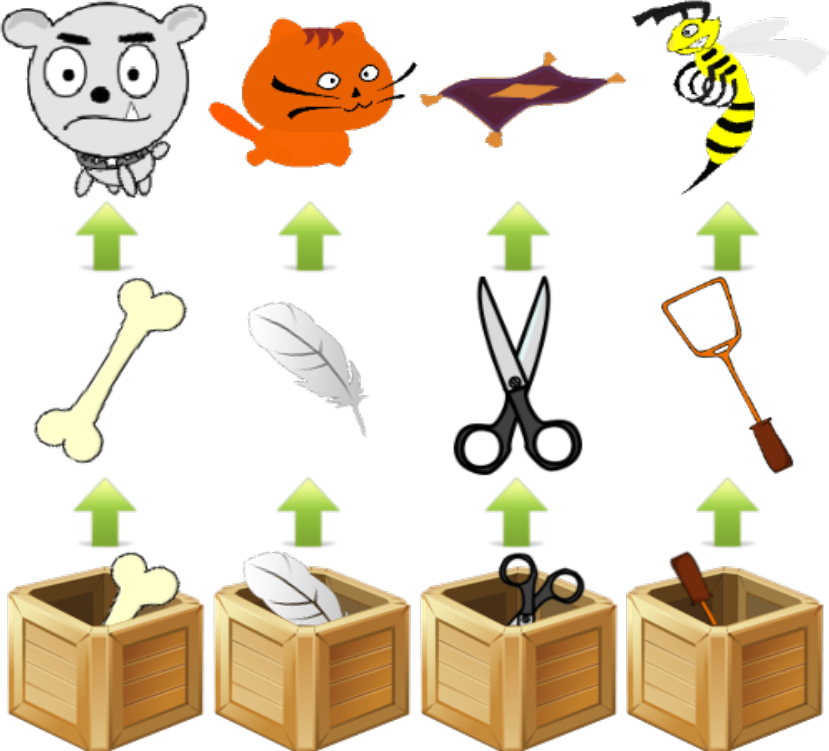
\includegraphics[scale=0.23]{images/esthetique.png}
\end{center}
\end{frame}

\begin{frame}
\frametitle{Plusieurs esthétiques : le lapin}
\begin{center}
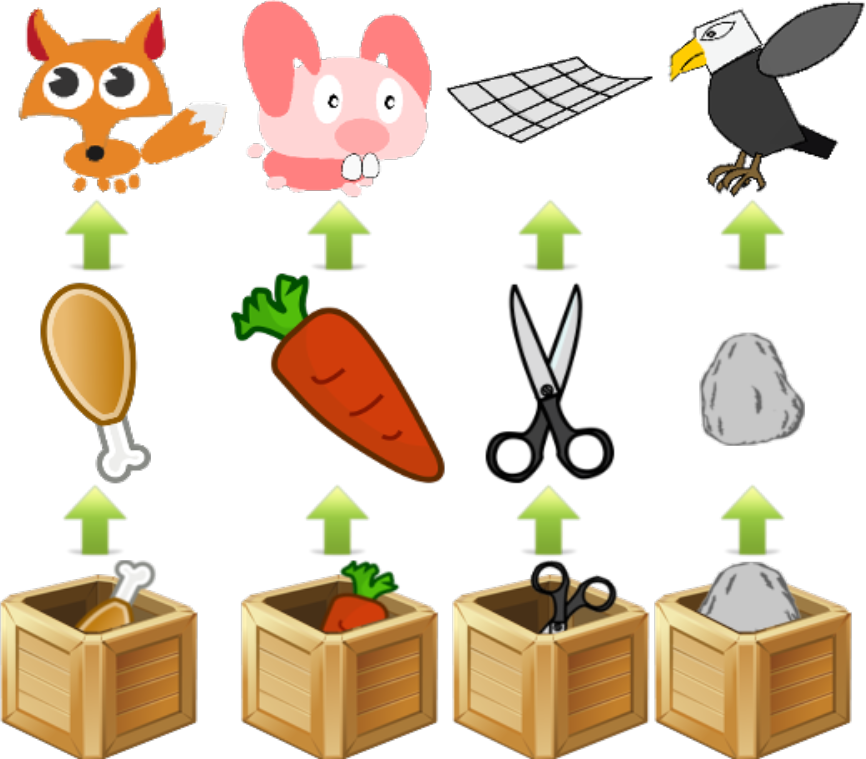
\includegraphics[scale=0.23]{images/esthetique1.png}
\end{center}
\end{frame}

\begin{frame}
\frametitle{Plusieurs esthétiques : la tortue}
\begin{center}
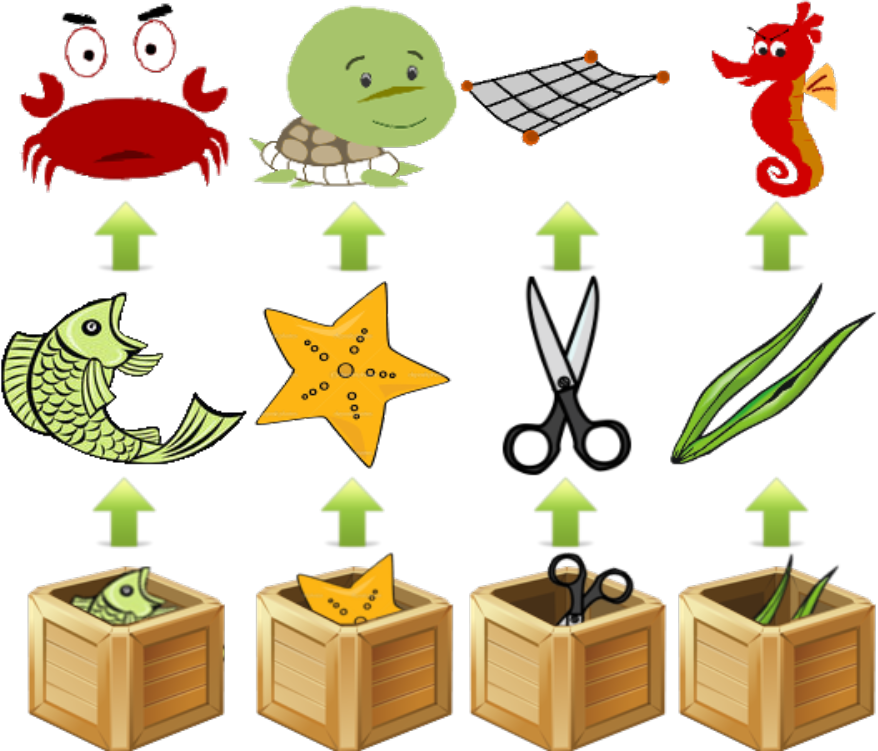
\includegraphics[scale=0.23]{images/esthetique2.png}
\end{center}
\end{frame}

\section{Résultats}

\subsection{Démonstration}
\begin{frame}
\frametitle{Démonstration du jeu}
\href{run:jar/rollingcat}{\beamerbutton{Rollingcat}}
\end{frame}

\subsection{En cours de test}
\begin{frame}
\frametitle{En cours de test...}
Le jeu est en test sur des patients depuis le 10 juin au Grau du roi jusqu'à la fin de la semaine. Il pourra ensuite être utilisé par les thérapeutes lors des séances de rééducation
\end{frame}

\begin{frame}
\frametitle{En cours de test...}
\begin{center}
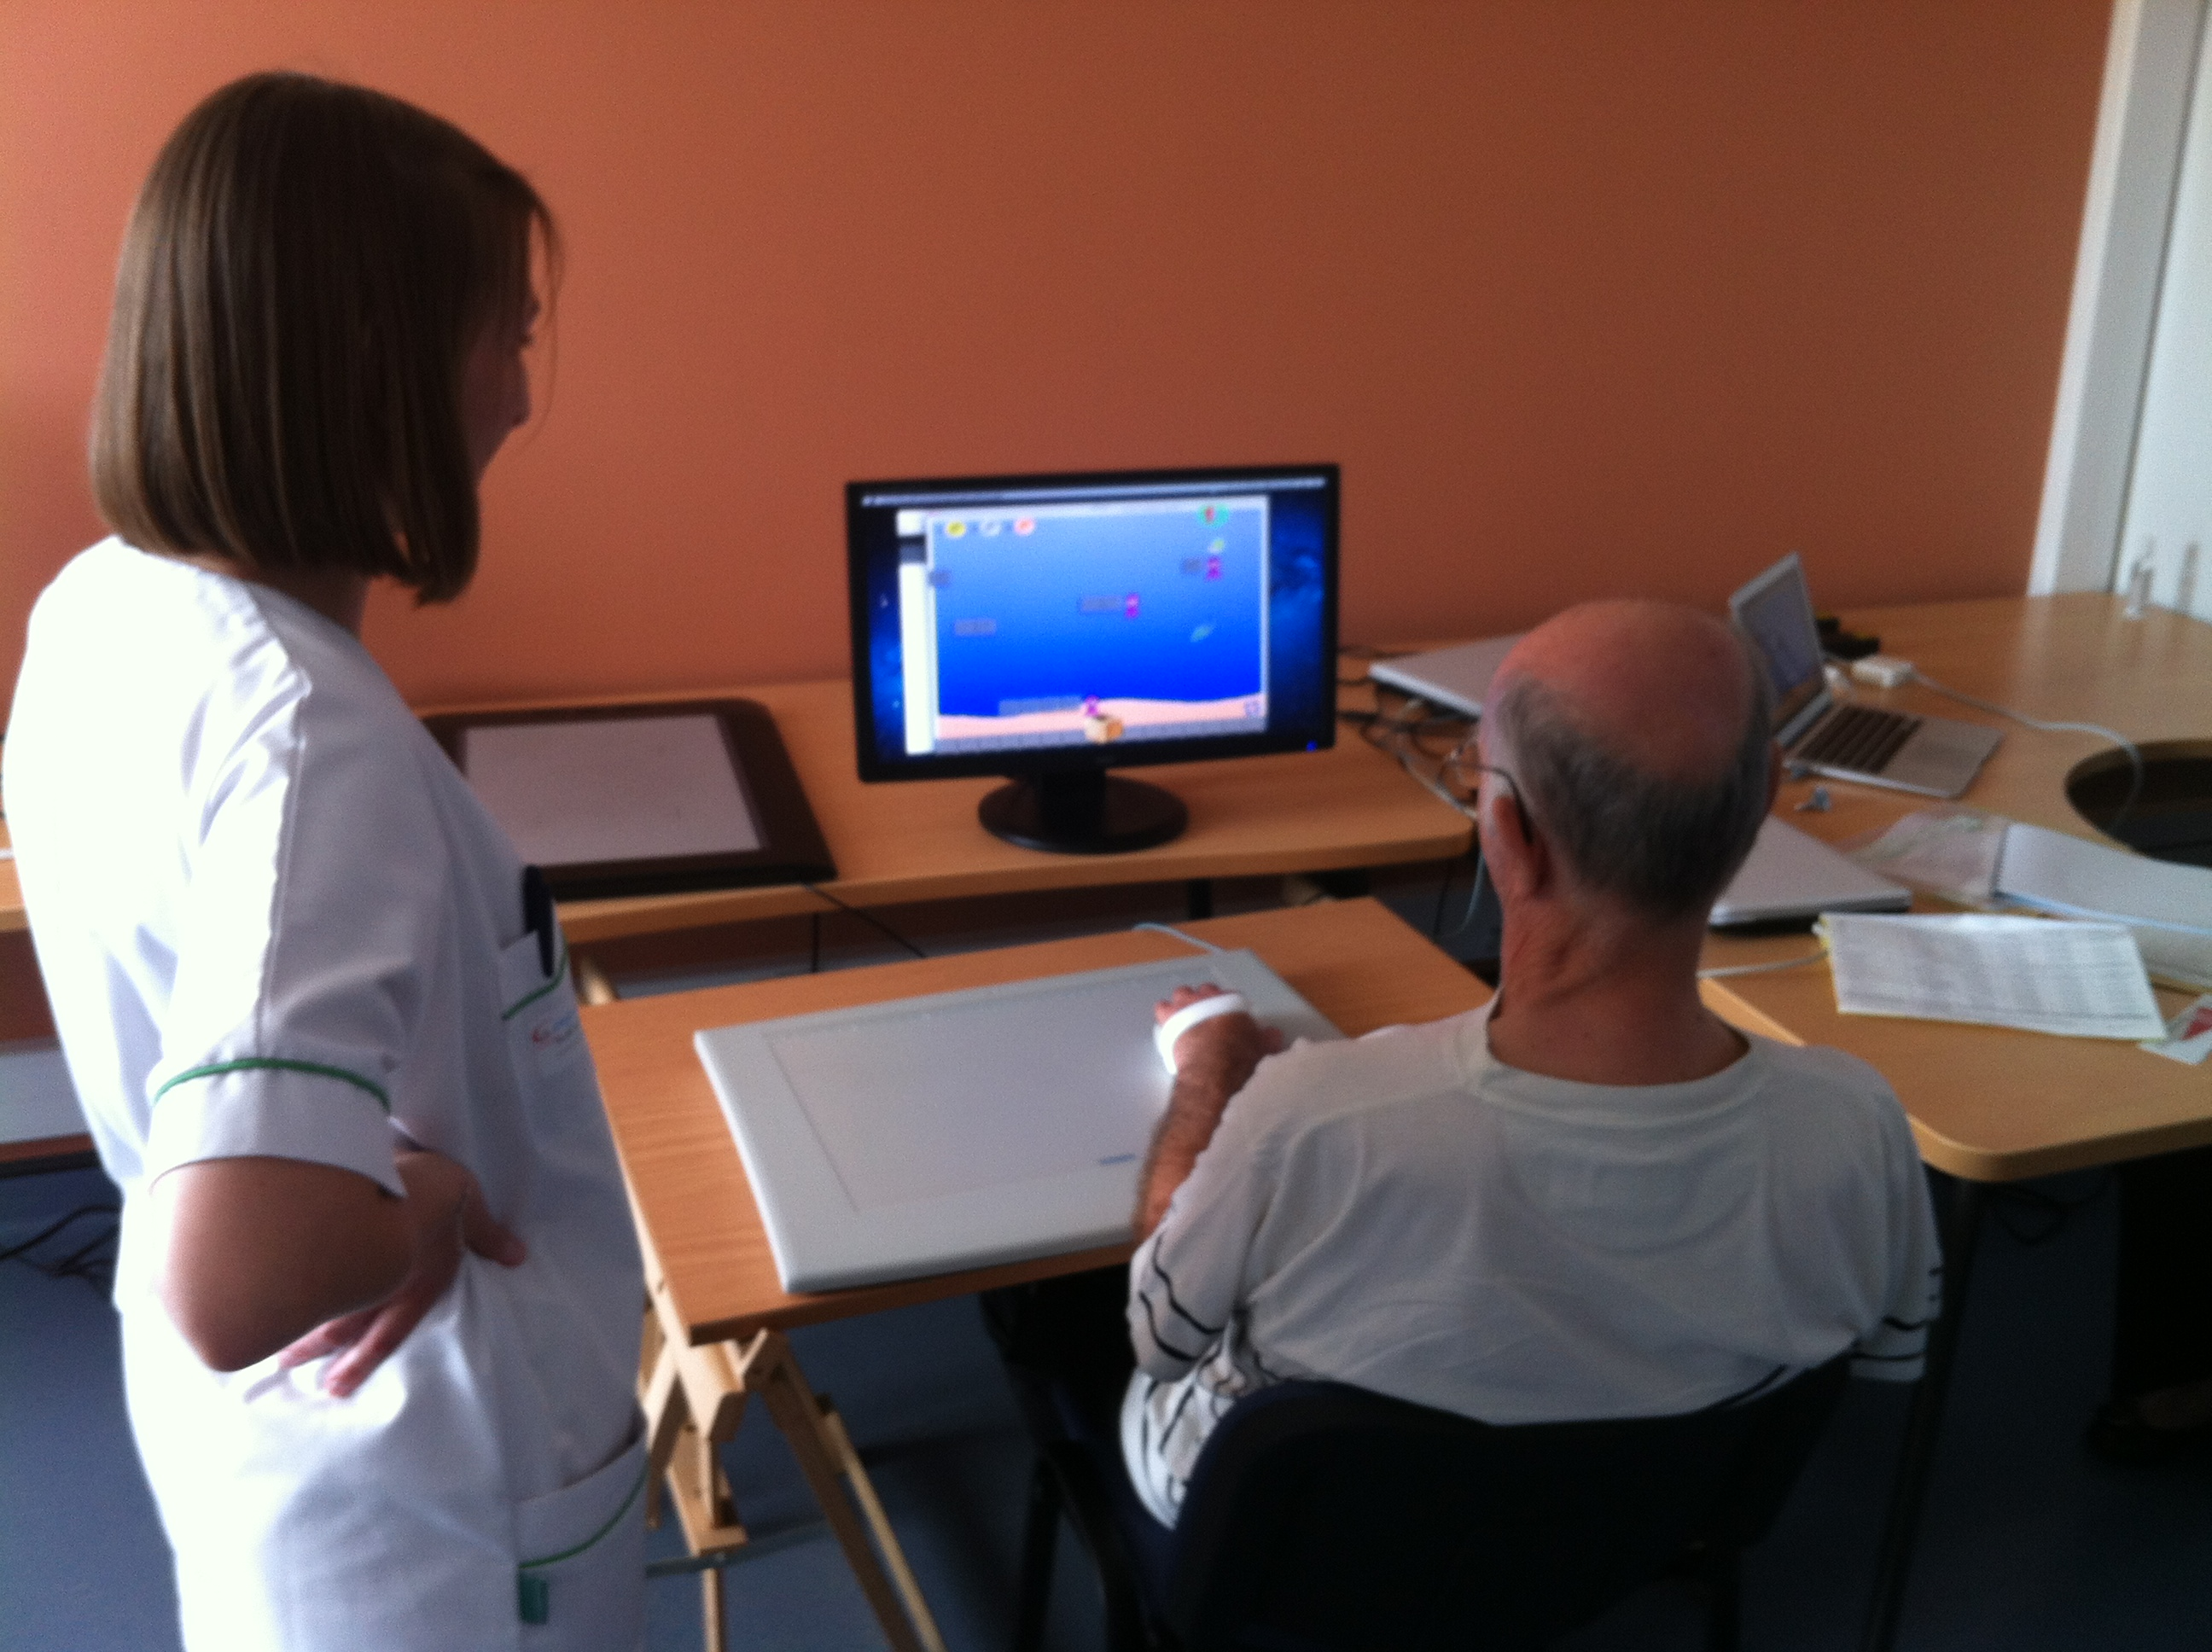
\includegraphics[scale=0.08]{images/test.JPG}
\end{center}
\end{frame}

\section{Conclusion}
\begin{frame}
\frametitle{Conclusion}
\begin{itemize}
\item Apprentissage d'un nouvel outil : LibGDX
\item Création d'un jeu de A à Z
\item Discipline qui touche la santé et l'informatique
\end{itemize}
\end{frame}


\end{document}
